\section{Implementation}\label{sec:trans_implementation}
Armed with the specifications and design decisions discussed in Section \ref{sec:trans_theory} it is time to step into the implementation phase. In practice this process is iterative, and the demands sometimes change with issues that emerge while working. This section aims to explain this process and describe some of the iterative steps that were taken.


\subsection{General structure}
To first gain an overview of how the transport layer protocol is implemented, the general design structure is going to be clarified in the following. When first beginning the process of writing code, two main entities were identified. One is the protocol system itself, and other the packet data structure. These two are implemented as the C++ classes \custtt{DtmfTransport} and \custtt{Packet}.

The \custtt{DtmfTransport} class takes care of the connection and most of the features described in the design specifications. It is both the interface to the rest of the system and the connection caretaker. To specify; \custtt{DtmfTransport} is essentially initiating, maintaining and closing connections - although it all happens on command of the user (through the API). The \custtt{DtmfTransport} class makes use of the services provided by the \custtt{Packet} class to be able to set up, and manipulate, packet data structures.

\custtt{Packet} directly represents the packet format as it is specified in Section \ref{sub:trans_packet_format}, meaning it basically consists of 8 bytes of header and up to 248 bytes of data. Add to that, a number of member functions are used to access or manipulate private members. The most important of these methods is probably \custtt{make()}, which is used to delay the initialization of the object members. Thus, packet objects can in fact be passed around while their data fields are empty.


\subsection{Function classification}
To better explain which member functions are doing what, they are split into two classifications: Core- and compatibility functions. The core functions are the ones providing functionality by directly implementing features that are described in the protocol design section. Compatibility functions are functions which are added to make the protocol compatible with other parts of the networking system.

\begin{table}[htb]
 \centering
 \begin{tabular}{lll}
  %      & \multicolumn{2}{c}{l}\\
  Class                    & Core methods                     & Compatibility methods              \\
  \midrule
  \smalltt{DtmfTransport}  & \smalltt{encode()}               & \smalltt{toPacketFromApi()}   \\
                           & \smalltt{decode()}               & \smalltt{packetFromCharBuffer()}   \\
                           & \smalltt{setPort()}              & \smalltt{packetToCharBuffer()}     \\
                           & \smalltt{connect()}              &                                    \\
                           & \smalltt{close()}                &                                    \\
                           & \smalltt{port()}                 &                                    \\
                           & \smalltt{connStatus()}           &                                    \\
  %
  \smalltt{Packet}         & \smalltt{make()}                 & \smalltt{makeFromArrays()}         \\
                           & \smalltt{calcChecksum()}         &                                    \\
                           & \smalltt{flagSet()}              &                                    \\
                           & \smalltt{orderBySeq::operator()} &                                    \\
 \end{tabular}
 \caption{Transport layer protocol member function classification}
 \label{tab:trans_function_classification}
\end{table}

Table \ref{tab:trans_function_classification} shows a list of member functions. Note that not all member functions, that are in the source files, are listed. Those not listed are merely specialized versions of other functions, or functions to access private member data (doing nothing else). As such they are not of great interest. The essential functions will be described more thoroughly in the following text, while the compatibility functions will only be touched briefly: They are mainly to fetch data out of buffers, to format data in a certain ways or to convert between object types. Yet they are important to mention.


\subsection{Main protocol interface}
As the protocol will need to function well with other parts of the networking system, the interface to it is of great import. The other layers are developed simultaneously, therefore having well-defined interfaces - even before implementation is undertaken - is essential. Otherwise one might risk incompatibility. To accomplish the goal of creating a good interface to the protocol, the two \custtt{encode()} and \custtt{decode()} are created as members of \custtt{DtmfTransport}. These methods were the first part of the transport layer protocol to be defined. This happened in collaboration with all the team members. The rest of the protocol is built based on these interface functions.

\begin{figure}[htb]
 \centering
 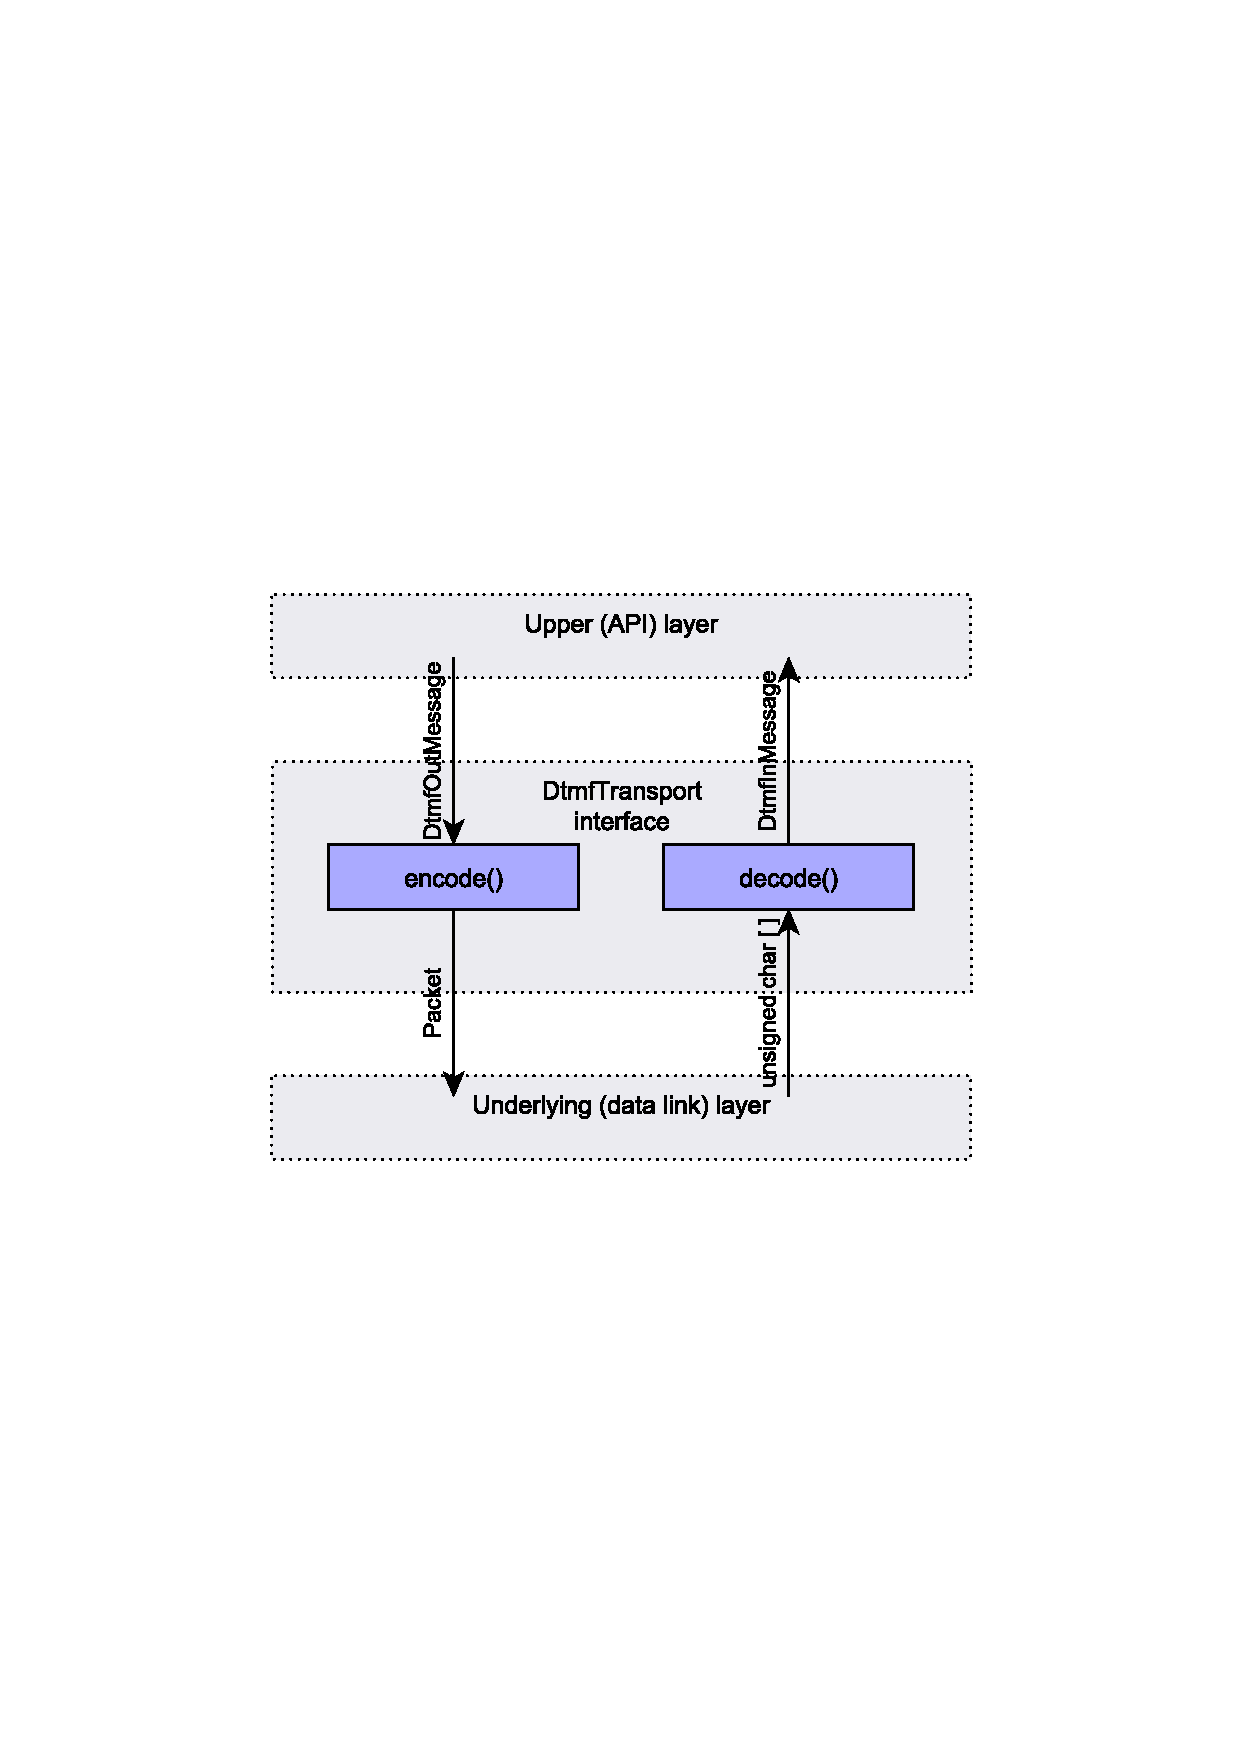
\includegraphics[scale=0.66,trim=0 280 0 275]{content/graphics/transport/trans_encode_decode.pdf}%trim=l b r t
 \caption{The transport layer protocol main interface methods}
 \label{fig:trans_encode_decode}
\end{figure}

Figure \ref{fig:trans_encode_decode} shows the \custtt{encode()} and \custtt{decode()} functions, and what in- and output they expect from the above API, and the underlying data link layer.


\subsection{Making a connection}
Wub


\subsection{Encoding messages from the API}
To first elaborate on the function of the \custtt{encode()} method, we see that it requires a message in the form of a \custtt{DtmfOutMessage} object, as described in more detail in Section \ref{sub:api_method_description}\marginnote{Verify ref.}. This message object from the API contains the receivers port number as well as a pointer to an array of data. This is the data we want cut into pieces of the right size, to enclose in the \custtt{Packet} object.

The compatibility method \custtt{toPacketFromApi()} serves as a tool to create a suitable number of packets. Only the destination port and data fields are initialized at this point, though. The packet does not yet contain all the header information needed to send it. \custtt{toPacketFromApi()} places the created packets in the FIFO queue \custtt{outQueue\_}.

\begin{figure}[htb]
 \centering
 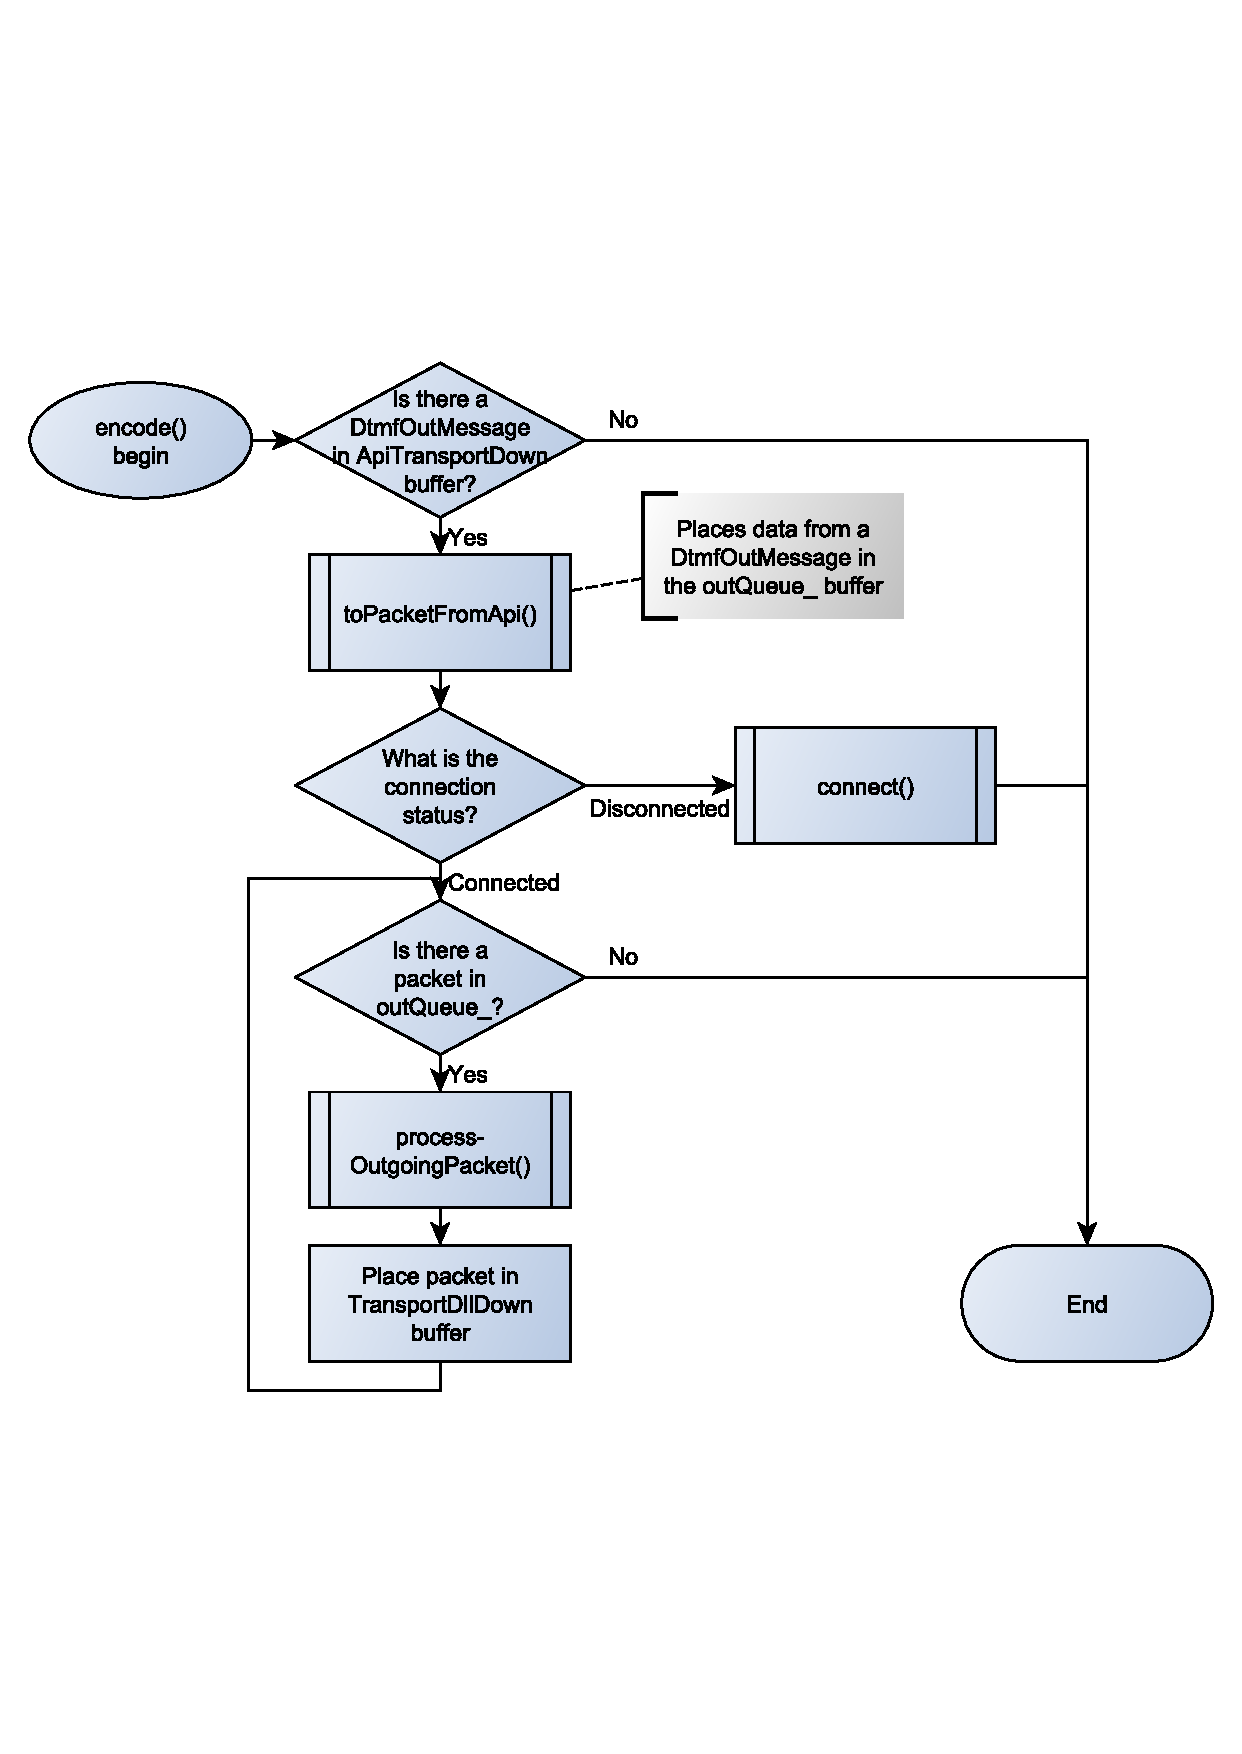
\includegraphics[scale=0.66,trim=0 207 0 205]{content/graphics/transport/trans_encode_flowchart_simple.pdf}%trim=l b r t
 \caption{The transport layer protocol encode function (simplified)}
 \label{fig:trans_encode_flowchart_simple}
\end{figure}

Figure \ref{fig:trans_encode_flowchart_simple} shows a simplified flowchart of the protocol encode function. It is seen how the rest of the header fields are filled by \custtt{DtmfTransport} automatically without user interaction. If the connection status is not read as ''connected'', the first packet to be sent is a SYN packet, where the sequence number is randomly generated - the \custtt{connect()} function takes care of that. If the connection is already established, the data packets queued by \custtt{toPacketFromApi()} will be sent (to the \custtt{TransportDllDown} buffer which the data link layer protocol reads from) with an appropriate sequence- and acknowledgment number. The source port number is set to the sender \custtt{DtmfTransport}'s port number as default, but can be changed.


\subsection{Decoding messages from the data link layer}
The method to pass data from the data link layer to the transport layer protocol, is chosen to simply be an array of bytes. These bytes are stored in a buffer. A pointer to this buffer is then passed on to the transport protocol, so that it can be read. It is then the protocols responsibility to make sense of this array of bytes. This is done via the \custtt{packetFromCharBuffer()} method, which is a member of \custtt{DtmfTransport}. It examines the buffer to see if there is enough data to make out the header: If there is, the packet header will be assembled to find out exactly what kind of response should be triggered.

